\documentclass[12pt, a4paper]{report}

\usepackage{amsmath,amsthm,amssymb}
\usepackage{mathtext}
\usepackage[T1,T2A]{fontenc}
\usepackage[utf8]{inputenc}
\usepackage[english,russian]{babel}
\usepackage{listings}
\usepackage{graphicx}
\usepackage{tablefootnote}
\usepackage{indentfirst}
\usepackage{color}
\usepackage{float}
\usepackage{caption}
\captionsetup[table]{singlelinecheck=off}
\captionsetup[lstlisting]{singlelinecheck=off, labelformat=empty}
\usepackage{pgfplots}
\pgfplotsset{compat=1.9}
\usepackage[left=3cm,right=1cm, top=2cm,bottom=2cm,bindingoffset=0cm]{geometry}
\graphicspath{{./img/}}

% Настройка заголовков
\makeatletter
\renewcommand\LARGE{\@setfontsize\LARGE{20pt}{30}}
\renewcommand\Large{\@setfontsize\Large{16pt}{20}}
\renewcommand\large{\@setfontsize\large{14pt}{20}}
\makeatother
\RequirePackage{titlesec}
\titleformat{\chapter}{\LARGE\bfseries}{\thechapter}{14pt}{\LARGE\bfseries}
\titleformat{\section}{\Large\bfseries}{\thesection}{14pt}{\Large\bfseries}
\titleformat{\sub}{\large\bfseries}{\thesubsection}{14pt}{\large\bfseries}
\titlespacing{\chapter}{12.5mm}{-35pt}{40pt}
\titlespacing{\section}{12.5mm}{20pt}{20pt}
\titlespacing{\subsection}{12.5mm}{10pt}{10pt}

\lstset{ 
	backgroundcolor=\color{white},   % choose the background color; you must add \usepackage{color} or \usepackage{xcolor}; should come as last argument
	breaklines=true,                 % sets automatic line breaking
	captionpos=t,                    % sets the caption-position to bottom
	commentstyle=\color{green},    % comment style
	keywordstyle=\color{blue},       % keyword style
	language=C++,                 % the language of the code
	numbers=left,                    % where to put the line-numbers; possible values are (none, left, right)
	numbersep=5pt,                   % how far the line-numbers are from the code
	numberstyle=\small\color{black}, % the style that is used for the line-numbers
	showspaces=false,                % show spaces everywhere adding particular underscores; it overrides 'showstringspaces'
	showstringspaces=false,          % underline spaces within strings only
	showtabs=false,                  % show tabs within strings adding particular underscores
	stepnumber=1,                    % the step between two line-numbers. If it's 1, each line will be numbered
	stringstyle=\color{yellow},     % string literal style
	tabsize=2,	                   % sets default tabsize to 2 spaces
	frame=single
}

\begin{document}
	
	\begin{titlepage}
		\noindent \begin{minipage}{0.15\textwidth}
			
\includegraphics[width=\linewidth]{bauman_image.jpg}
		\end{minipage}
		\footnotesize\noindent \begin{minipage}{0.8\textwidth}\centering
			\textbf{Министерство науки и высшего образования Российской Федерации}\\
			\textbf{Федеральное государственное бюджетное образовательное учреждение}\\
			\textbf{высшего образования}\\
			\textbf{~~~«Московский государственный технический университет}\\
			\textbf{имени Н.Э.~Баумана}\\
			\textbf{(национальный исследовательский университет)»}\\
			\textbf{(МГТУ им. Н.Э.~Баумана)}
		\end{minipage}
		
		\noindent\rule{17cm}{3pt}
		\newline\newline
		\large\noindent ФАКУЛЬТЕТ $\underline{\text{Информатика и системы управления}}$ \newline\newline
		\noindent КАФЕДРА $\underline{\text{Программное обеспечение ЭВМ и информационные технологии}}$\newline\newline\newline\newline\newline
		
		
		\begin{center}
			\noindent
			\LARGE\textbf{Отчёт по домашнему заданию}\newline
			\textbf{по дисциплине "Анализ алгоритмов"}\newline\newline
		\end{center}
		
		\large\noindent\textbf{Тема} $\underline{\text{Графовые модели}}$\newline\newline
		\noindent\textbf{Студент} $\underline{\text{Жабин Д.В.}}$\newline\newline
		\noindent\textbf{Группа} $\underline{\text{ИУ7-54Б}}$\newline\newline
		\noindent\textbf{Преподаватель} $\underline{\text{Волкова Л.Л.}}$\newline\newline\newline
		
		\begin{center}
			\large\vfill
			Москва, 2021 г.
		\end{center}
	\end{titlepage}
	
	\setlength{\parindent}{1.25cm}
	\setcounter{page}{2}\large\linespread{1.3}
	
	\newpage
	\chapter*{Код алгоритма}
	
	В листинге 1 приведен исследуемый фрагмент кода.
	
	\begin{lstlisting}[title=Листинг 1~--- Код алгоритма,firstnumber=0]
std::vector<Pixel> ZBuffer::calculatePixels(Polygon &polygon, int minX, int maxX, int minY, int maxY) {
	std::vector<Pixel> ans;
	ActivePolygon activePolygon(polygon);
	for (int scanlineY = polygon.getY(); scanlineY <= polygon.getY() + polygon.getDeltaY() && scanlineY <= maxY; scanlineY++) {
		activePolygon.check(scanlineY);
		if (scanlineY >= minY) {
			Segment segment = activePolygon.segment();
			ActiveSegment activeSegment(segment);
			for (int scanlineX = segment.getX(); scanlineX <= segment.getX() + segment.getDeltaX() && scanlineX <= maxX; scanlineX++) {
				if (scanlineX >= minX) {
					float z = activeSegment.getZ();
					QVector3D p = activeSegment.getP(), n = activeSegment.getN();
					QColor color = calculateColor(p, n);
					ans.push_back(Pixel(scanlineX, scanlineY, z, color));}
				activeSegment.update();}}
		activePolygon.update();}
	return ans;}
	\end{lstlisting}

	\chapter*{Графовые модели}
	
	На рисунках 1 -- 4 представлены 4 графовые модели, описывающие приведенный фрагмент кода: операционный граф, операционная история, информационный граф и информационная история соответственно. Для построения операционной и информационной историй рассмотрим следующий случай:
	
	\begin{itemize}
	\item пусть значение maxY такое, что всегда scanlineY <= maxY;
	\item пусть значение minY такое, что всегда scanlineY >= minY;
	\item пусть значение maxX такое, что всегда scanlineX <= maxX;
	\item пусть значение minX такое, что всегда scanlineX >= minX.
	\end{itemize}
	
	\begin{figure}[H]
		\center{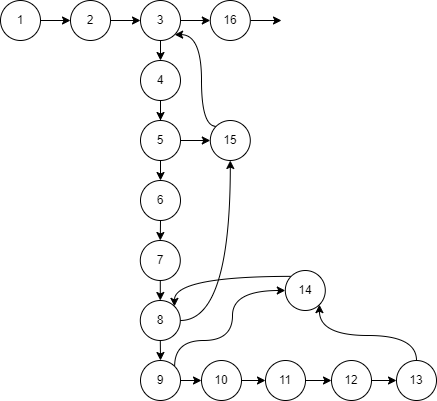
\includegraphics[scale=0.8]{opgraph.png}}
		\caption*{Рисунок 1~--- Операционный граф}
	\end{figure}

	\begin{figure}[H]
		\center{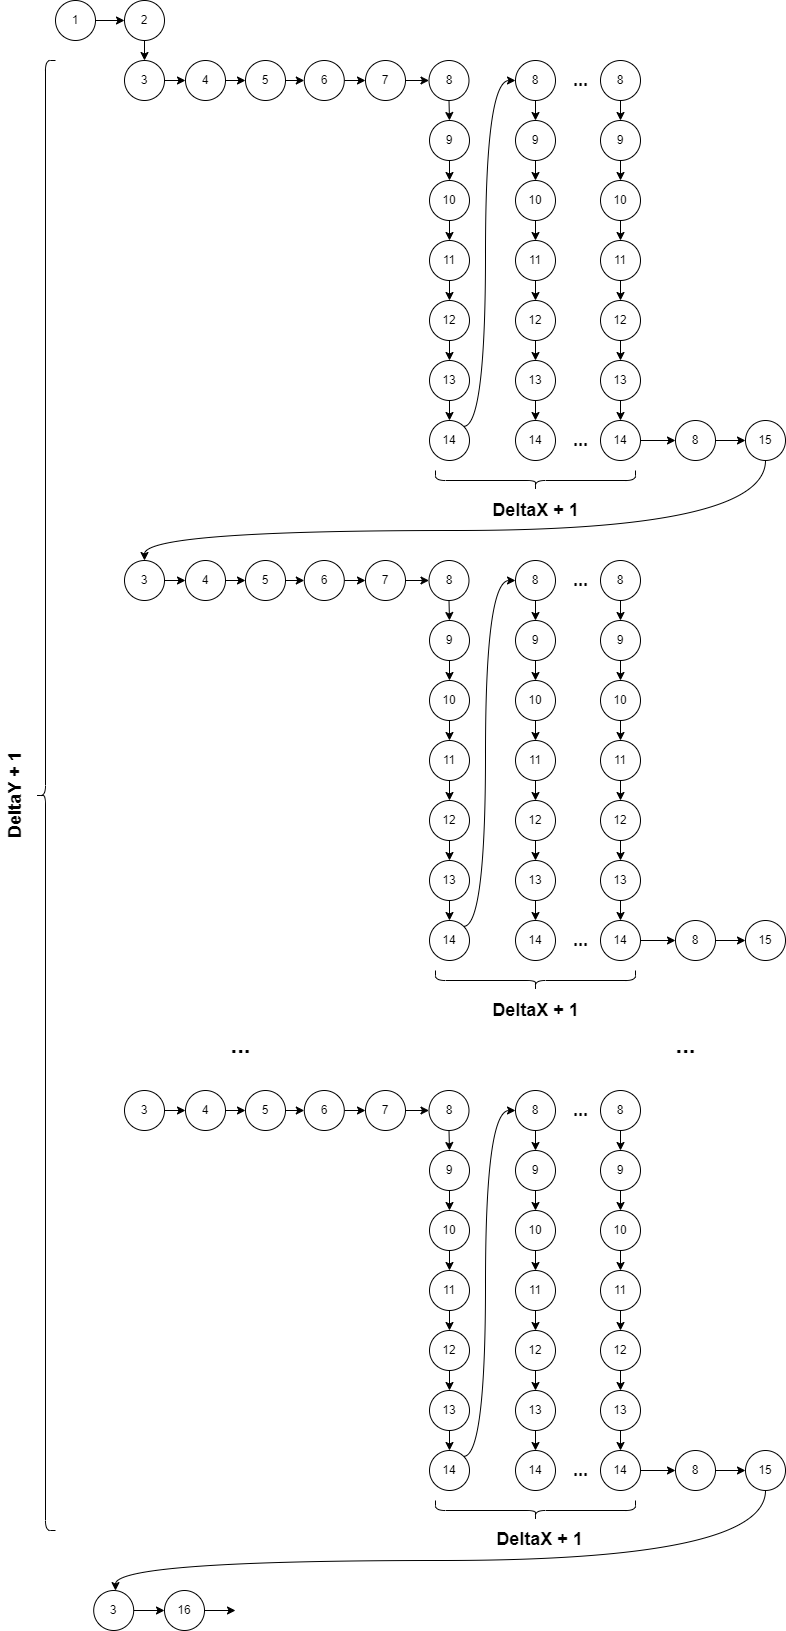
\includegraphics[scale=0.44]{opstory.png}}
		\caption*{Рисунок 2~--- Операционная история}
	\end{figure}

	\begin{figure}[H]
		\center{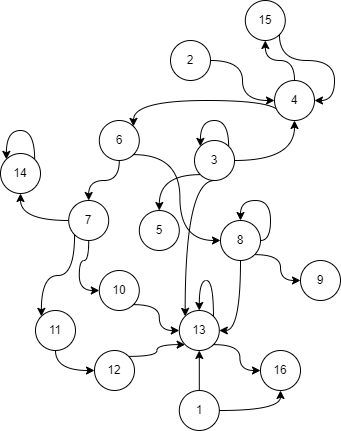
\includegraphics[scale=0.8]{infgraph.png}}
		\caption*{Рисунок 3~--- Информационный граф}
	\end{figure}

	\begin{figure}[H]
		\center{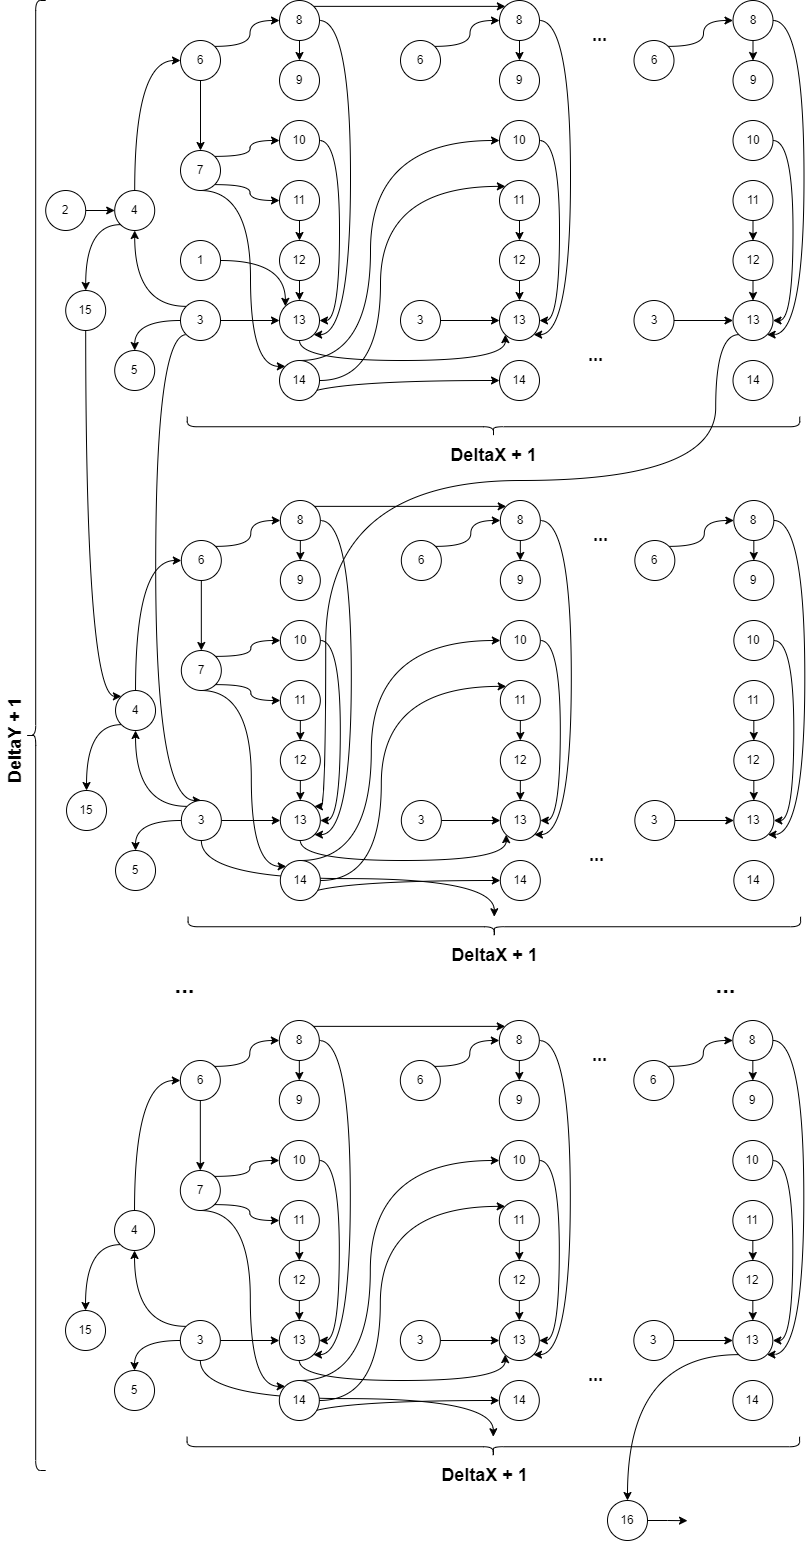
\includegraphics[scale=0.46]{infstory.png}}
		\caption*{Рисунок 4~--- Информационная история}
	\end{figure}
	
\end{document}